\documentclass[compress,11pt]{beamer}
%\includeonly{pendel}
\usetheme{Ilmenau}
%\usetheme{fau-4-3}
%\usecolortheme{beaver}
%\beamertemplatenavigationsymbolsempty
\usepackage[ngerman]{babel}
\usepackage{marvosym}
\usepackage{multimedia}
\usepackage[utf8]{inputenc}
\usepackage{amsmath}
\usepackage{amsfonts}
\usepackage{amssymb}
\usepackage{graphicx}
\usepackage{esvect}
%\author{}
\title{EP Gruppe 8}
%\setbeamercovered{transparent}
%\setbeamertemplate{navigation symbols}{}
%\logo{}
%\institute{}
%\date{}
%\subject{}
\usepackage{verbatim}
\begin{document}

\frame[c]{\titlepage}
\begin{frame}
\tableofcontents
\end{frame}

\section{Aufgabe 1}
\subsection{a)}
\begin{frame}{Innenwiderstand}
\begin{block}{Shuntwiderstand im DMM}
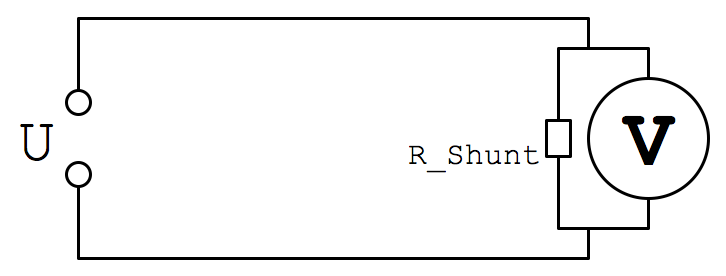
\includegraphics[width=\textwidth]{images/1a.png} %Schaltbild
\end{block}
\end{frame}

\begin{frame}
Tabellen Widerstände U|I|R
\end{frame}

\begin{frame}
%Messpunkte ohne Fit
%\includegraphics[width=\textwidth]{images/4/double-pendulum}
\end{frame}


\begin{frame}
\begin{block}{Was fällt auf?}
\begin{itemize}
\item Klicken im Messgerät an gleichen Stellen, wie Änderung des Innenwiderstands
\item 
\end{itemize}
Innenwiderstand des Messgeräts ändert sich, um größere Messbereiche abdecken zu können.
\end{block}
\end{frame}


\begin{frame}
Ein großer Strom fliest nur dann, wenn der Widerstand des Schaltkreises gering ist. Ein großer Messwiderstand hätte daher einen zu großen Anteil am Gesamtwiderstand.\\
Damit auch bei kleinen Strömen eine messbare Spannung abfällt, muss der Shunt-Widerstand entsprechend vergrößert werden.
\end{frame}
\subsection{b}
\begin{frame}
\sunsection{NPLC=1,n=3000}
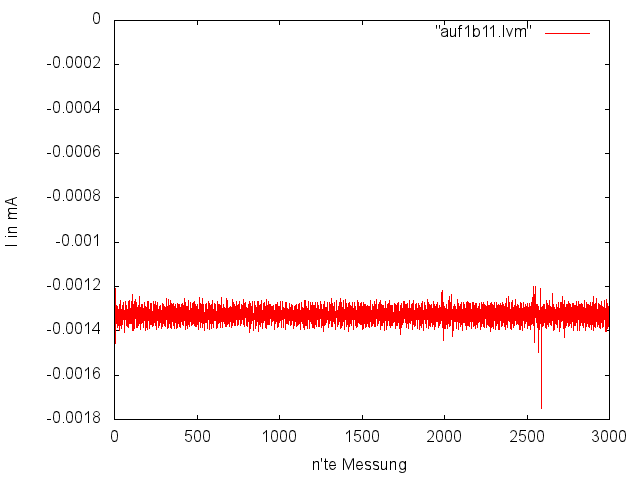
\includegraphics[width=\textwidth]{images/auf1b11_lines.png}

\end{frame}
\begin{frame}
\subsection{NPLC=1,n=3000, Power-Supply lief vor Messbeginn}
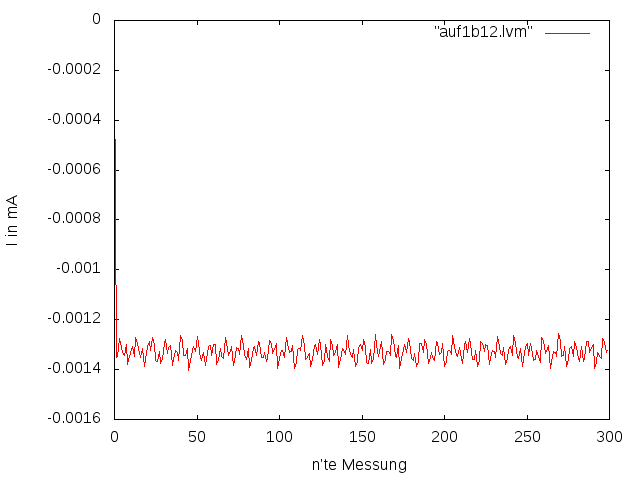
\includegraphics[width=\textwidth]{images/auf1b12_lines.png}
Aufnahme 1 rauscht, aufnahme 2 nicht. Das liegt daran, dass die Transistoren im Power-Supply erst warm laufen müssen. 
\end{frame}
\begin{frame}
\tiny
\begin{tabular}{|c|c|c|c|c|}
\hline 
Integrationszeit & Mittel & Standardabweichung & Minimum & Maximum \\ 
\hline 
• & -1.2058e-04 & 1.61212e-06 & -1.2800e-04 & -1.1500e-04 \\ 
\hline 
• & -0.00133 & 7.56109e-05 & -0.00141 & -1.85000e-04 \\ 
\hline 
• & -0.0072289 & 0.011962 & -0.027426 & 0.014268 \\ 
\hline 
• &  -0.013617 & 0.012539 &  -0.036758 & 0.009862 \\ 
\hline 
• & -0.01734781 & 0.0129556 & -0.041245 &  0.006758 \\ 
\hline 
• & -0.0161734 & 0.012837 & -0.040475 & 0.008057 \\ 
\hline 
• & -9.6051465e-04 & 0.002076 & -0.004252 & 0.0023890 \\ 
\hline 
\end{tabular} 
\end{frame}

\begin{frame}
%\includegraphics[width=\textwidth]{images/4/tracker}
\end{frame}

\section{Aufgabe 2}

\subsection{Schaltung 1}
\begin{frame}
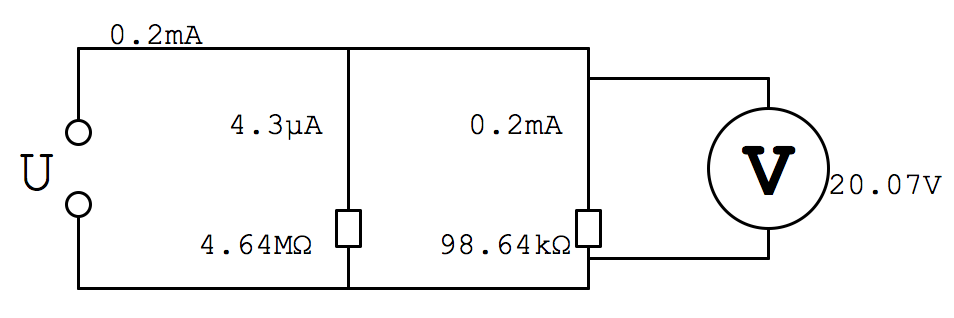
\includegraphics[width=\textwidth]{images/21.png}
\end{frame}
\begin{frame}
\subsubsection{Widerstände}

Alle Werte sind in $\Omega$ angegeben. Für die berechneten Widerstände wurden die an den jeweiligen Stromstärken verwendet.\\
\begin{tabular}{|c|c|c|c|}
\hline 
- & Erwarteter Widerstand & Berechneter " & Gemessener " \\ 
\hline 
$R_{ges}$  & 97916.7 & 100000 & 96586.7 \\ 
\hline 
$R_1$ & 4700000 & 4652790.7 & 4640000 \\ 
\hline
$R_2$ & 100000 & 100035 & 98640 \\
\hline
\end{tabular}

\subsubsection{Stromstärken an den Widerständen}
Erhält man über den folgenden Ansatz:
\begin{equation}
U = const. = I_1 \cdot R_1 = I_2 \cdot R_2
\end{equation}
\begin{equation}
\Rightarrow \frac{I_1}{I_2} = \frac{R_2}{R_1} = \frac{1 k\Omega}{4.7 M\Omega} = \frac{1}{47}
\end{equation}
\begin{equation}
I_{ges} = I_1 + I_2 = \frac{I_2}{47} + I_2
\end{equation}
\begin{equation}
\Rightarrow I_2 = \frac{47}{48} \cdot I_{ges} = \frac{47}{48} \cdot 0.2 mA = 1.9583 e-4
\end{equation}
\begin{equation}
I_1 = I_{ges} - I_2 = 4.167 \mu A
\end{equation}
Werte stimmen bis auf kleine Ungenauigkeiten mit den gemessenen Werten überein.
\subsubsection{Leistung an den Widerständen}
\begin{equation}
P_1 = I_1^2 \cdot R_1 = 8.16 e-5 W
\end{equation}
\begin{equation}
P_2 = I_2^2 \cdot R_2 = 0.004 W
\end{equation}
\end{frame}

\subsection{Schaltung 2}
\begin{frame}
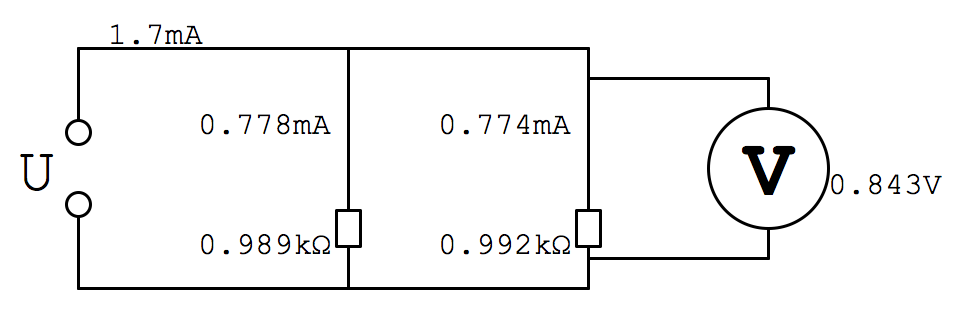
\includegraphics[width=\textwidth]{images/22.png}
\end{frame}
\begin{frame}
$R_{ges} = 500 \Omega$ \\ Mit $U_{ges,genmessen} = 0.843 V$ und $I_{ges,gemessen} = 1.7 mA$ ergibt sich: 
\begin{equation}
R_{ges} = \frac{U_{ges}}{I_{ges}} = 495.9 \Omega
\end{equation}
\begin{equation}
R_{1,gem} = 989 \Omega 
\end{equation}
\begin{equation}
R_{2,gem} = 992 \Omega
\end{equation}
\begin{equation}
\Rightarrow R_{ges,gem} = \frac{R_{1,gem} \cdot R_{2,gem}}{R_{1,gem} + R_{2,gem}} = 495.25 \Omega
\end{equation}
\end{frame}

\subsection{Schaltung 3}
\begin{frame}
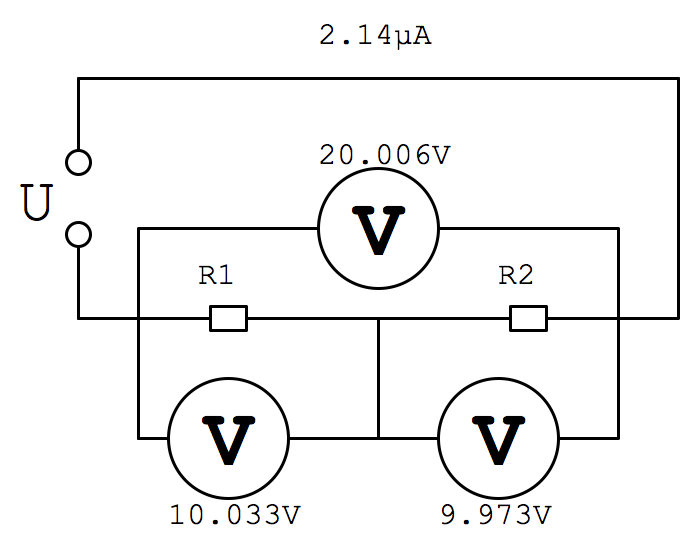
\includegraphics[width=\textwidth]{images/23.png}
\end{frame}
\begin{frame}
$R_{ges} = 9.4 M \Omega$, $I_{ges,gem} = 2.14 \mu A$, $U_{ges,gem} = 2.006 V$
Es ergibt sich:
\begin{equation}
R_1 = \frac{U_1}{I} = 3802336.5 \Omega
\end{equation}
\begin{equation}
R_2 = 3779906.5 \Omega
\end{equation}
Gemessene Widerstände sind zu klein, da der tatsächliche Widerstand des Stromkreises im Verhältnis zum Innenwiderstand des DMM zu groß ist, d.h. es fällt zu viel Spannung am DMM ab. Mit dem Modus "HI-Z" wird der Innenwiderstand auf 10 G$\Omega$ erhöht und es ergibt sich:
\begin{equation}
R_1^{(HI-Z)} = \frac{U_1^{(HI-Z)}}{I} = \frac{10.033 V}{I}= 4688317.8 \Omega
\end{equation}
\begin{equation}
R_2^{(HI-Z)} = \frac{9.937 V}{I}=4660280 \Omega
\end{equation}
\end{frame}

\section{Aufgabe 3}
\subsection{Widerstand $1k\Omega$}
\begin{frame}
Widerstand bei $100Hz$
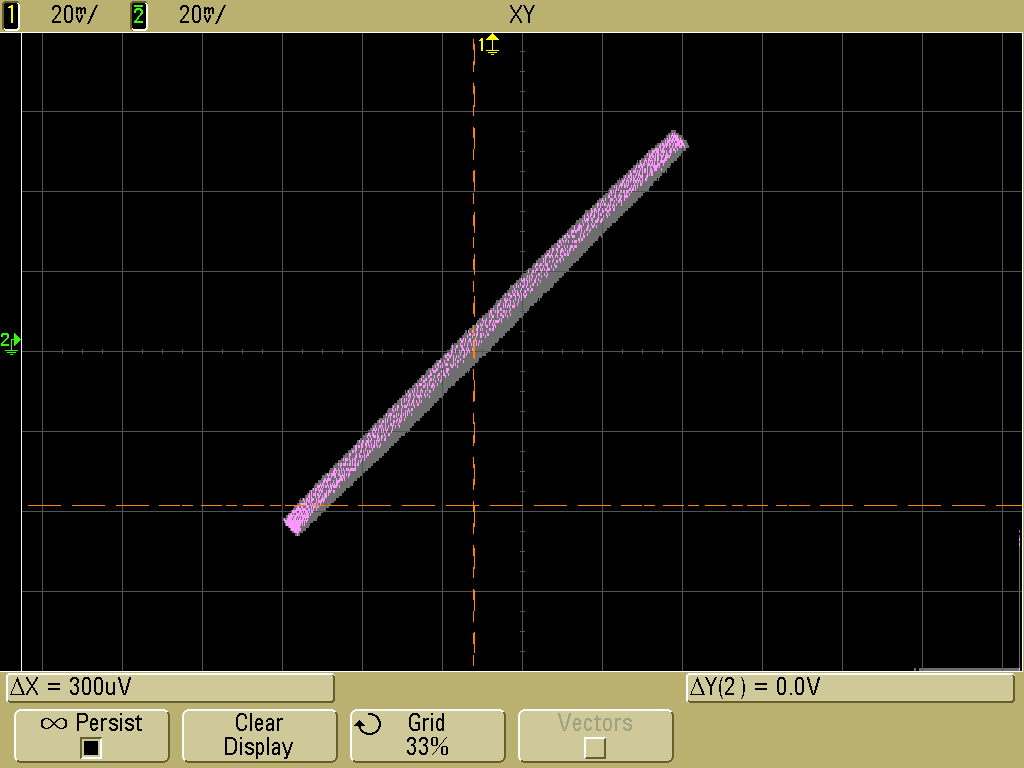
\includegraphics[width=\textwidth]{images/scope_5}
die Steigung der Geraden lässt auf einen Widerstand von $1k\Omega$ schließen
\end{frame}
\begin{frame}
Bei höheren Frequenzen bildet Sich eine Elipse. Hier der $1k\Omega$ Widerstand bei 1kHz
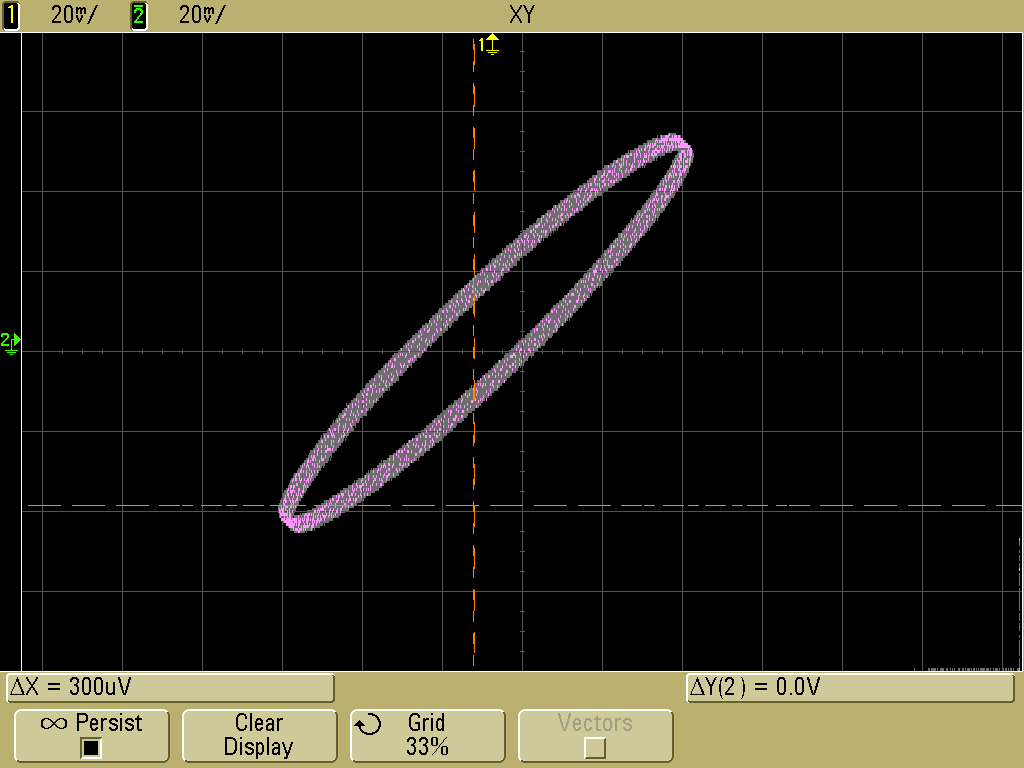
\includegraphics[width=\textwidth]{images/scope_6}
\end{frame}
\begin{frame}
Der Effekt, der nicht linearen Kennlinie bei einem einfachen Widerstand lässt sich durch die Verbindung von Funktionsgenerator und Oszilloskop über die Erde erklären.
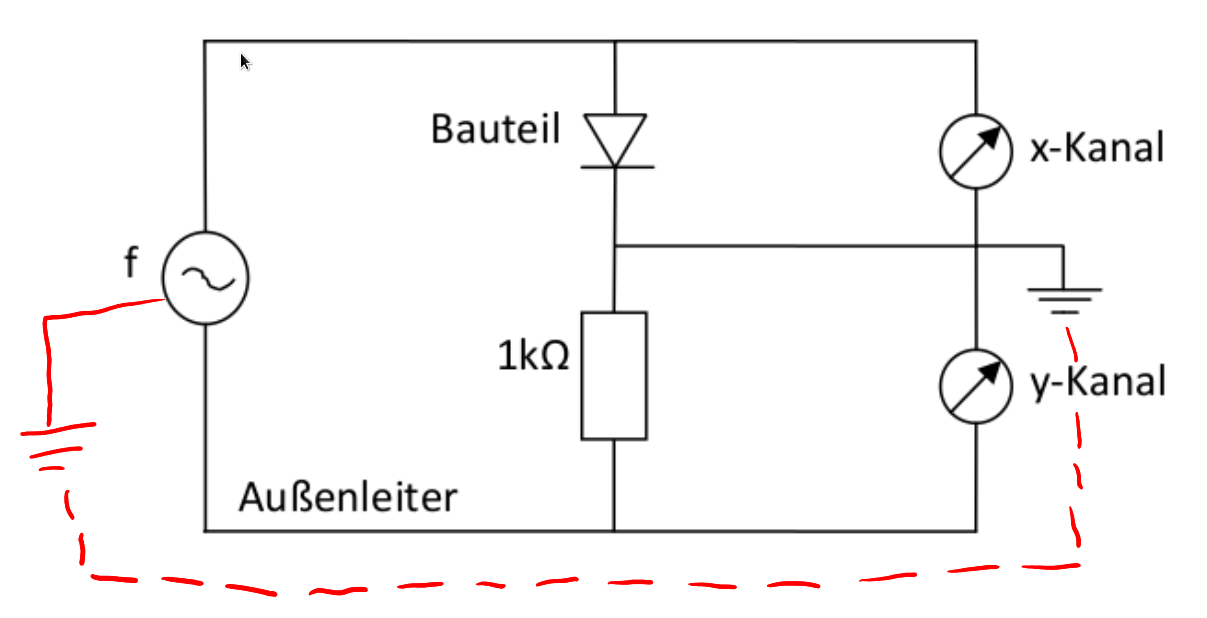
\includegraphics[width=\textwidth]{images/3-erde.png}
\end{frame}
\subsection{Weiße LED}
\begin{frame}
	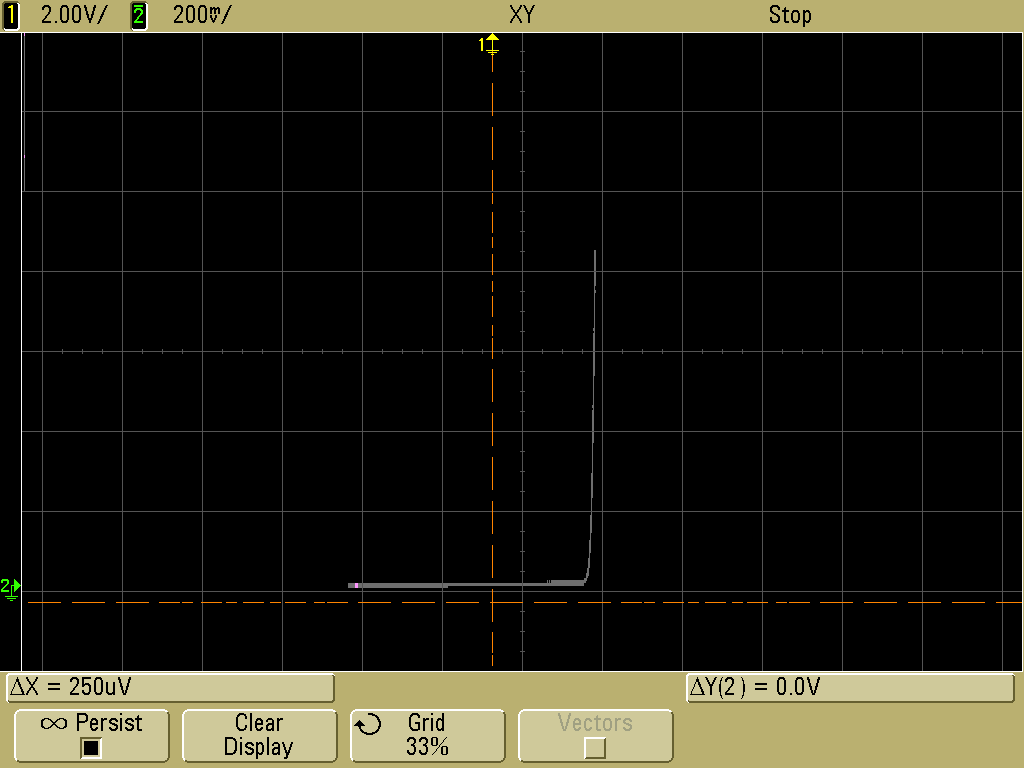
\includegraphics[width=.6\textwidth]{images/scope_8}\\
	Die weiße LED weist eine Durchlassspannung von $3V$ auf
\end{frame}
\subsubsection{Silizium Diode}
\begin{frame}
	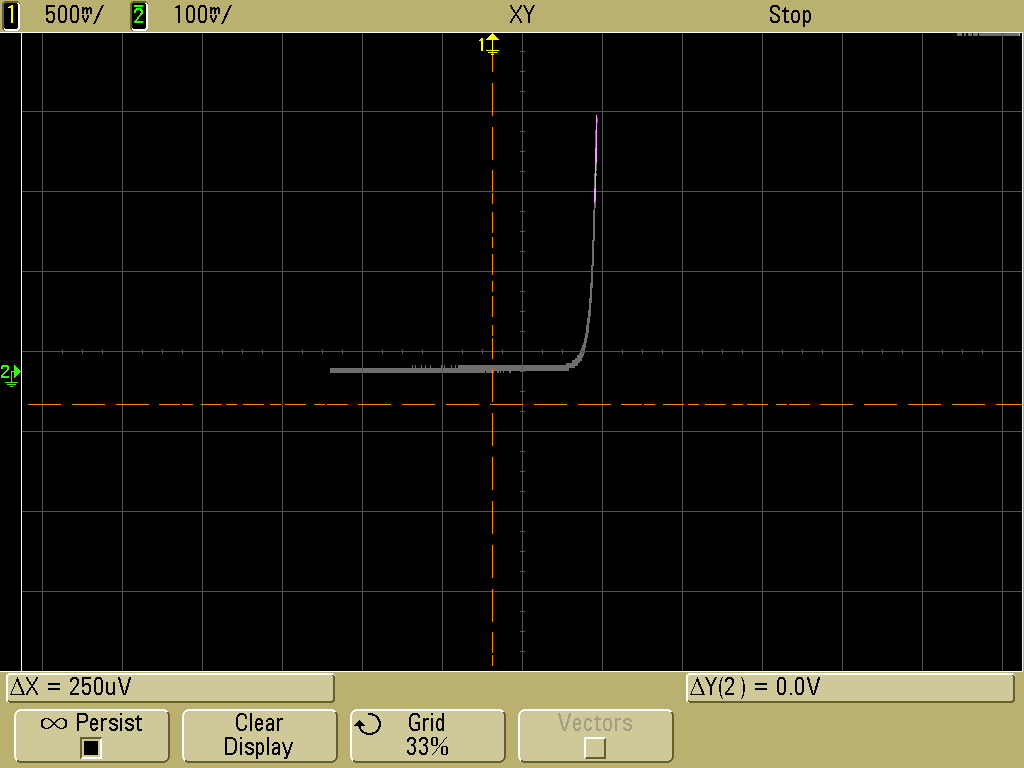
\includegraphics[width=.6\textwidth]{images/scope_11}\\
	Die Siliziumdiode weißt eine Duchlassspannung von $0.7V$ auf
\end{frame}
\section{Aufgabe 4}
\begin{frame}
\subsection{Eigenschaften des Signals}
Amplitude: $U_0 = 2.35625 V$ \\
Frequenz: $f = 59.172 kHz$ \\
Offset: $U_{off} \approx 0.1 V$
Phase: $U(t=0) \approx 0.09 V$\
\end{frame}

\begin{frame}
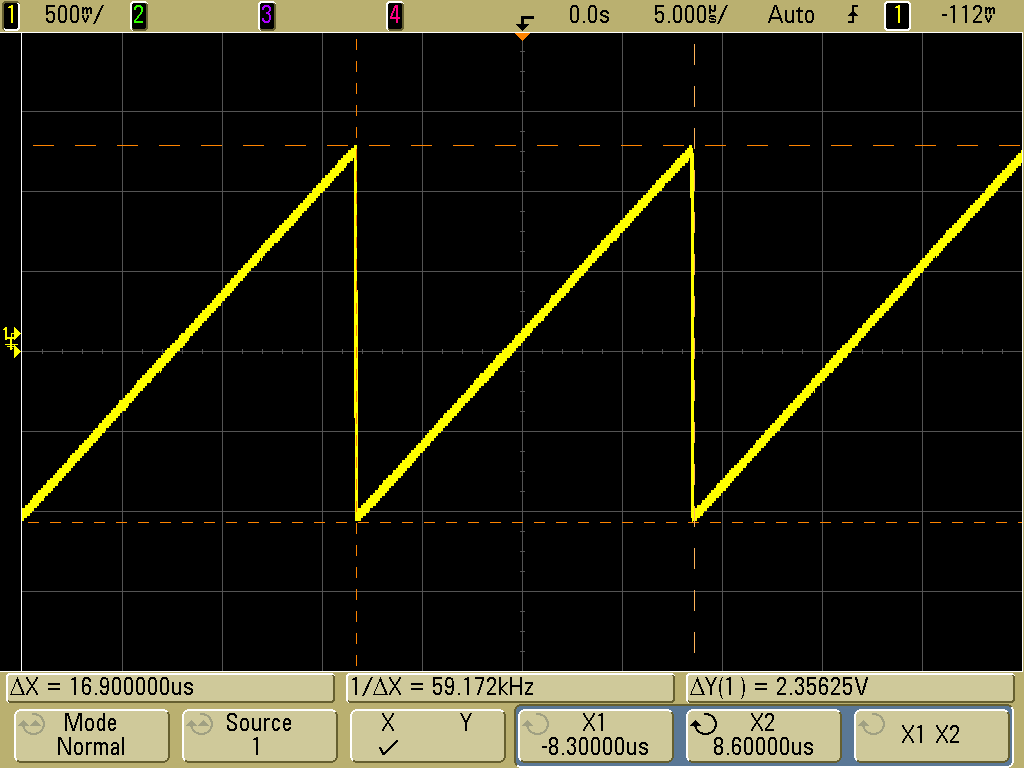
\includegraphics[width=\textwidth]{images/scope_13}
\end{frame}
\begin{frame}
\subsection{Eigenschaften des Signals}
Amplitude: $U_0 = 2.35625 V$ \\
Frequenz: $f = 59.172 kHz$ \\
Offset: $U_{off} \approx 0.1 V$ \\
Phase: $U(t=0) \approx 0.09 V$\
\end{frame}
\section{Aufgabe 5}
\subsection{Virtuelles Labor}
\begin{frame}
	Im Virtuellen Labor wurde festgestellt, dass einige Geräte zu Störungen in Form von scharfen Peaks im Spektrum führten.
\end{frame}
\begin{frame}\centering
	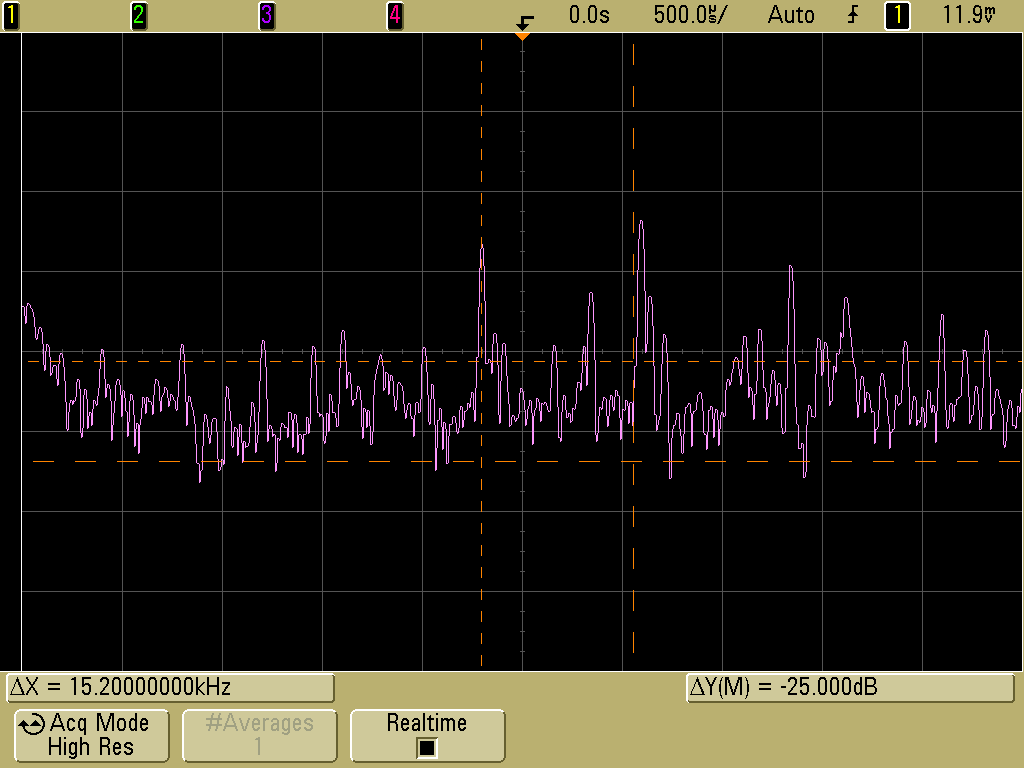
\includegraphics[width=.6\textwidth]{images/scope_15}\\
	Die im virtellen Labor simulierten Störungen des Frequenzgenerators konnten auch in einer Messung des Einflusses des Funktionsgenerators nachgewiesen werden. 
\end{frame}
\begin{frame}
Selbst bei Verwendung eines Koaxialkabels konnte ein Peak bei $50Hz$ festgestellt werden.
\centering
	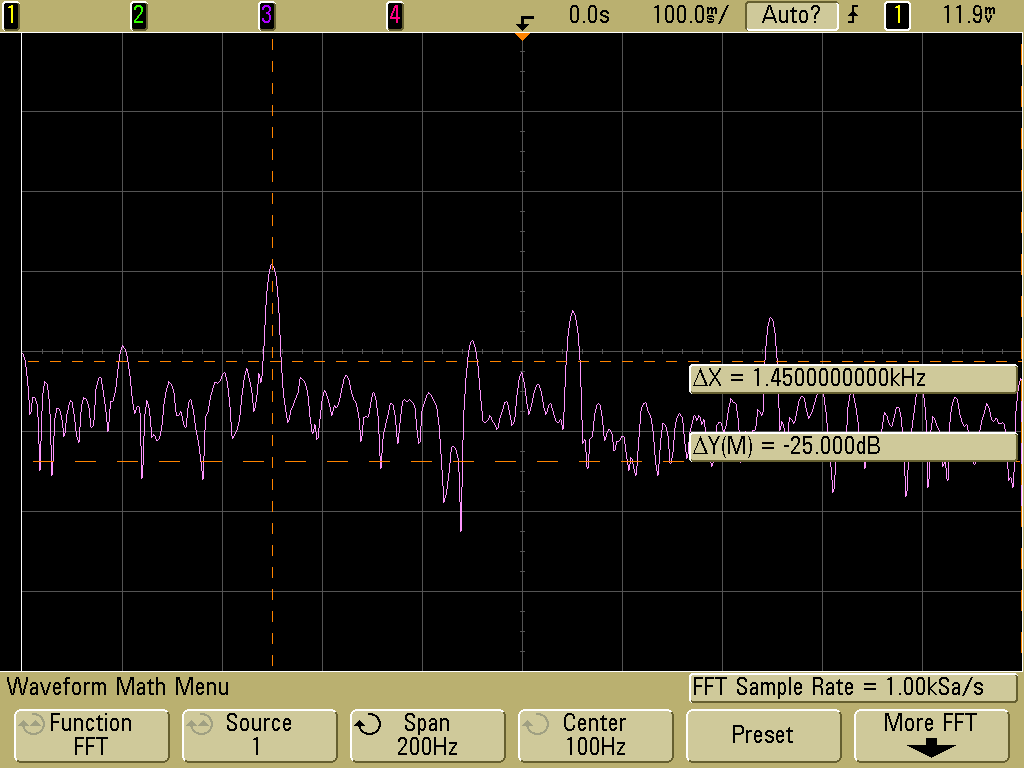
\includegraphics[width=.7\textwidth]{images/scope_16}	
\end{frame}
\end{document}
